%% question-2.tex
%%

%% ==============================
\subsection{Version enrichie du diagramme de classe du jeu}
\label{sec:question-2}
%% ==============================

Dans cette version du diagramme de classe \ref{fig:Jeu}, la classe Jeu est est maintenant associée a deux nouvelles classes.

La classe \emph{Position}, qui possède deux attributs positionX et positionY qui va conserver la position de chaque objet présent pendant le Jeu.

La classe \emph{Personnage}, qui représente les personnages (avatar ou zombie) avec leurs points de vie, leur ratio d'attaque et leurs effets et leur position. Cette classe à deux sous-classes :
\emph{Zombie} et \emph{Avatar}.

\emph{Avatar} comporte maintenant des aspects normaux et payants, une portée de visibilité, un ratio de défense et un nom. Cette classe est liée à \emph{Détail} qui va garder le détail des matchs et des
opposants rencontrés lors de ceux-ci. Elle est également liée à \emph{Stratégie} qui va contenir la stratégie à appliquer et.

\emph{Avatar} est aussi liée à \emph{Rencontre} vu qu'il est utilisé lors de celles-ci. Il possède un \emph{Inventaire}

\emph{Joueurs} est maintenant une classe abstraite contenant un pseudo et si il à payé pour des aspects suplémentaires. Ses deux sous-classes sont \emph{Physique} qui représente un joueur physique et 
\emph{Machine} qui représente une machine avec un niveau de difficulté.

L'\emph{Avatar} possède également un \emph{Inventaire} qui est composé d'une opération permettant d'ajouter un item à celui-ci. Cet \emph{Inventaire} possède dont des \emph{Objet}. Ces Objets peuvent être de 4
sous-classes. La première sous-classe \emph{Ramassable} qui peut-être \emph{Nourriture}, \emph{Boisson} et \emph{Munition}. La seconde sous-classe \emph{Orientation} qui peut être \emph{Carte} ou \emph{Radar}.
La troisième sous-classe \emph{Aide} Qui peut être un \emph{Activable} \emph{Cape} ou \emph{Cotte de maille}, Ou peut être \emph{Bottes pare-feu} \emph{Bottes à crampons} ou \emph{Kit de plongée}. La quatrième
sous-classe \emph{Bonus} qui peut être un \emph{BonusAttaque} ou \emph{BonusDefense}.

Au niveau de la classe \emph{Monde}, elle possède maintenant des \emph{Cases}, chacune d'entre elles sont en bas ou en haut d'une autre. A gauche ou a droite d'une autre. Chaque \emph{Cases} peut être vide ou
alors un \emph{Obstacle}, un \emph{Item} ou le \emph{Graal}. Si elle est un \emph{Obstacle}, celui-ci peut être une \emph{Zone} un \emph{Franchissable} ou un \emph{Infranchissable}.


\begin{sidewaysfigure}
    \centering
	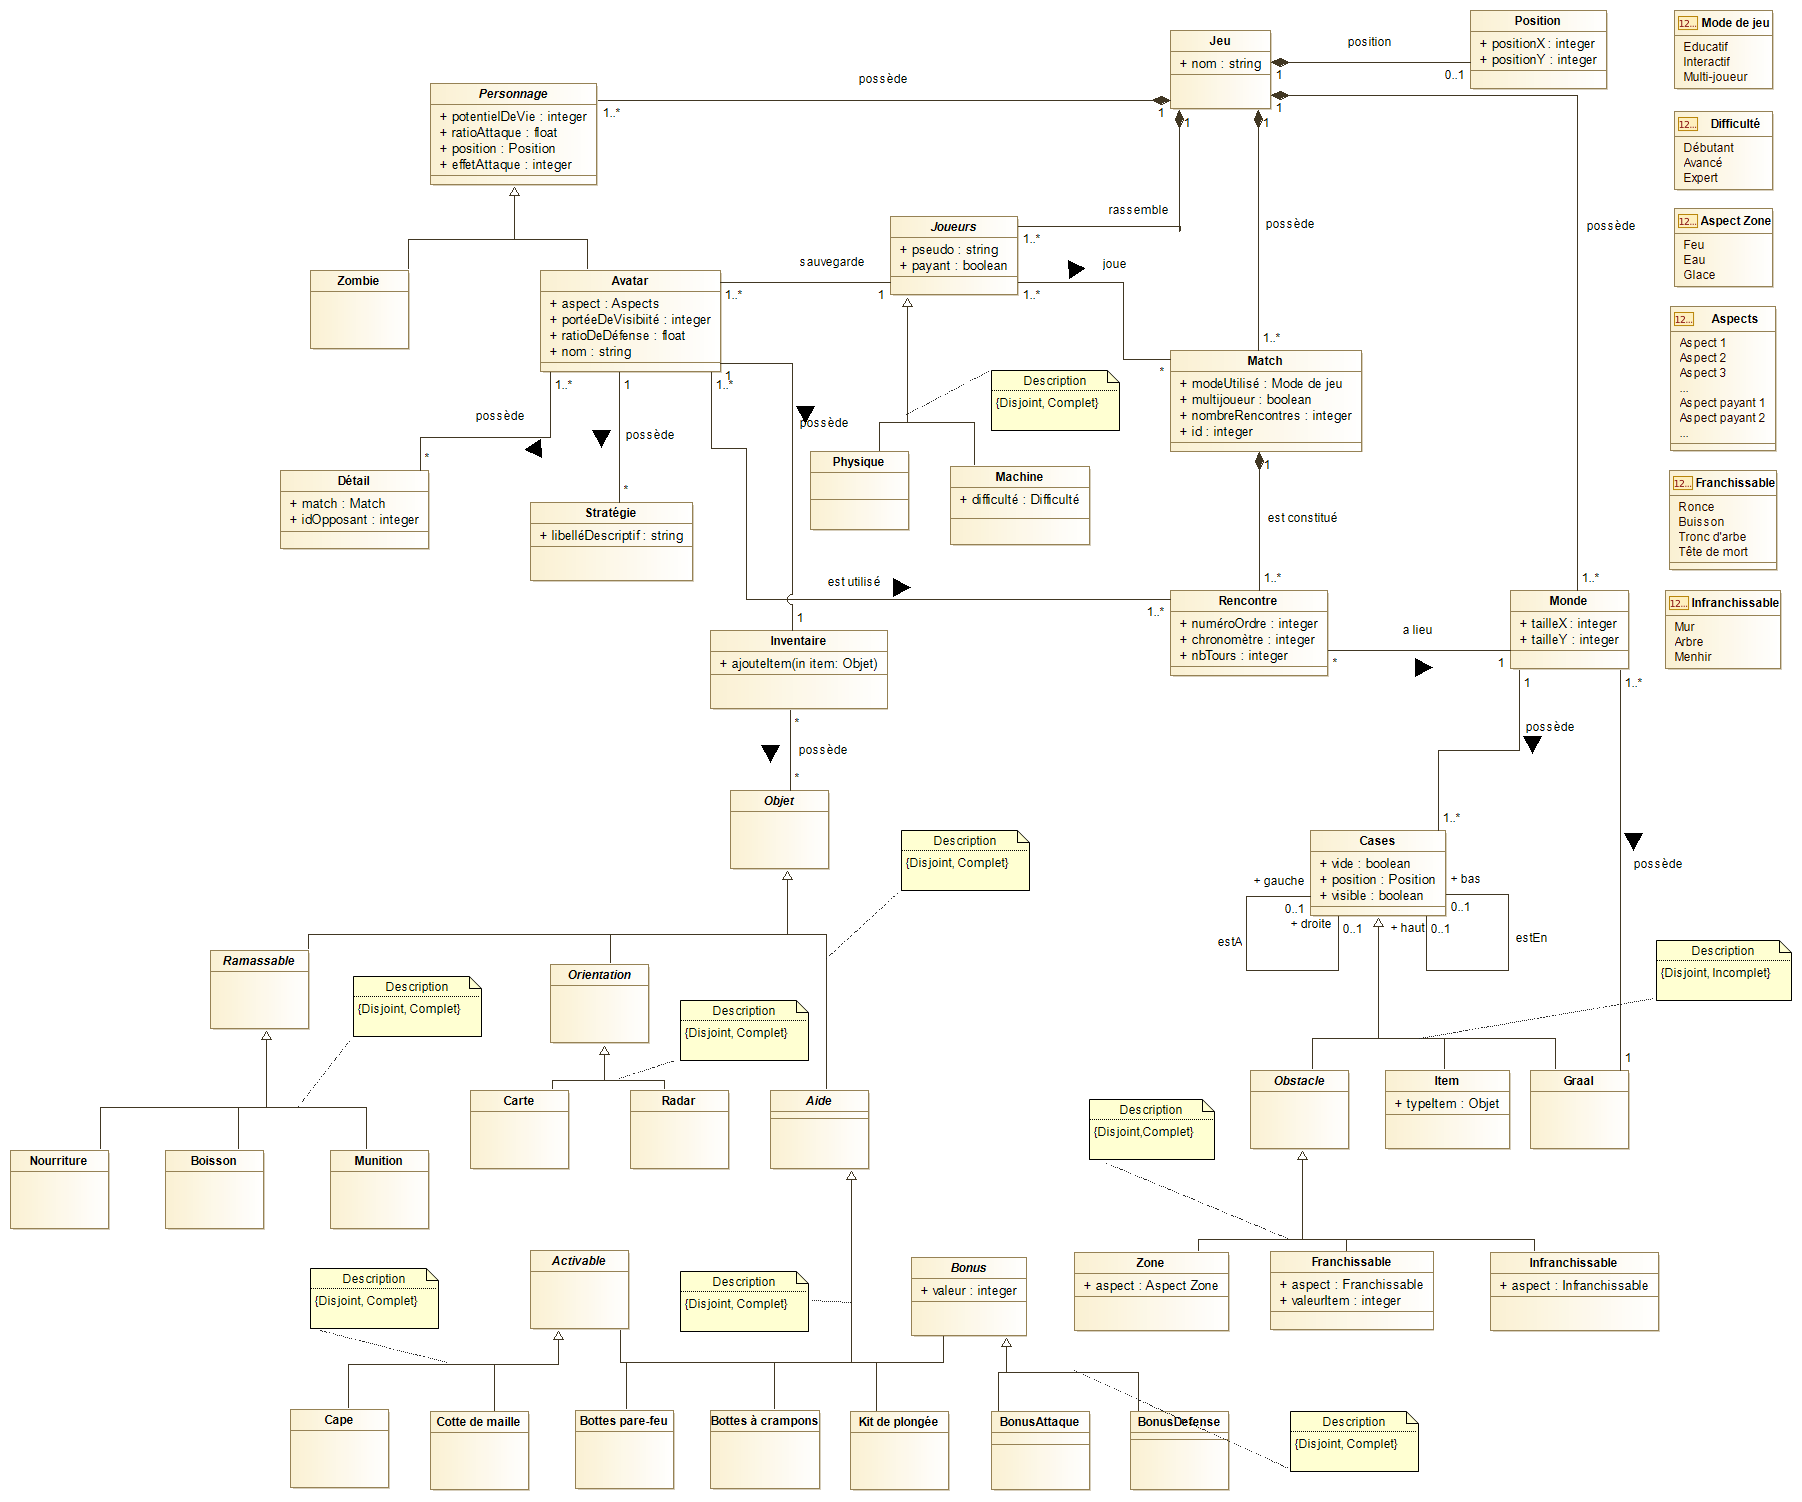
\includegraphics[width=\textwidth]{assets/Jeu}
	\caption{Diagramme enrichit}
	\label{fig:Jeu}
\end{sidewaysfigure}

\newpage